\documentclass[a4paper,10.5pt]{article}
\usepackage[a4paper, top=0.3in, bottom=1.4in, left=1.4in, right=1.4in]{geometry}
\usepackage{amsmath, amssymb, graphicx, hyperref}
\usepackage[utf8]{inputenc}
\usepackage{graphicx}
\usepackage{multimedia}
\usepackage{media9}
\graphicspath{{Images/}}
\usepackage{float}
\usepackage{tcolorbox} % Add this in the preamble

\title{Complex Differentiation and its Applications in Computational Fluid Dynamics}
\author{Datta Souvik \quad Irwin Kong \quad Liu Meichi \quad Liu Zichen}

\vspace{0.2cm}

\date{}

\begin{document}

\maketitle

\vspace{-1cm}
\begin{tcolorbox}[colframe=black, colback=gray!10, sharp corners=south]
\textbf{Problem Statement}
\vspace{0.2cm}

1. What does it mean to differentiate a function taking in a complex number and returning a complex result? \\
2. What mathematical challenges arise and what are the solutions to them? \\
3. What about a function that takes in a complex number and returns a real number? \\
4. How does one define the derivative of such a function?
\end{tcolorbox}

\section{Introduction}
How can we extend the concept of derivatives to functions that map between two-dimensional spaces? Understanding complex differentiation can be challenging, but a geometric approach helps make it more intuitive.

\vspace{0.25cm}
In this blog post, we will develop an intuitive understanding of complex differentiation by focusing on geometric transformations. We will explore how these derivatives function, visualize their effects, and examine their practical applications in computational fluid dynamics (CFD).
\vspace{0.25cm}

Our goal is to simplify the concept of complex differentiation while demonstrating its real-world importance.

\section{Complex Functions}
Complex functions map between two-dimensional spaces, taking a complex number as an input (with real and imaginary axes) to a complex number output, written mathematically as: $C \rightarrow C$. For a complex input $z = x + iy$, we can write the output as: $w = f(z) = u + iv$, where $u$ and $v$ are real-valued functions of $x$ and $y$.

For a specific $z$, this mapping can be visualized using two 2D graphs: one representing the input space and one representing the output space, as shown below:
\begin{figure}[H]
    \centering
    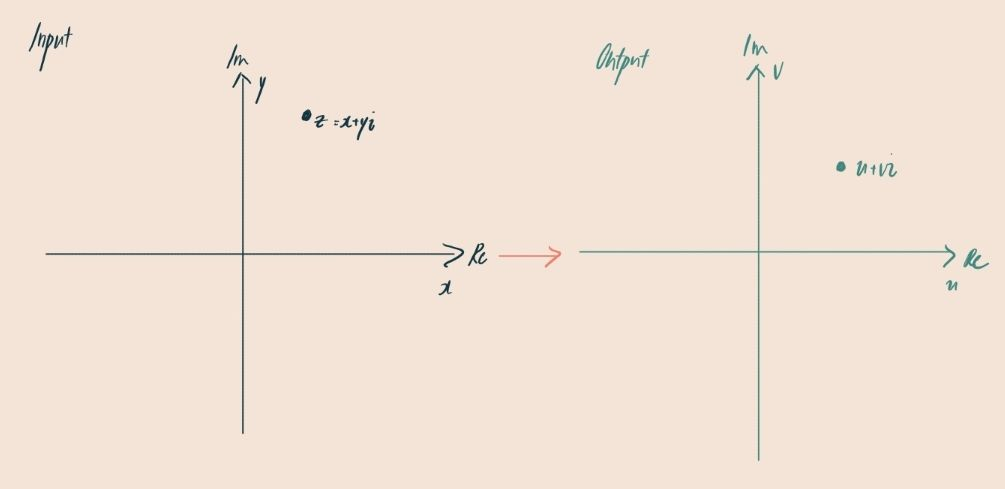
\includegraphics[width=0.8\textwidth, keepaspectratio]{Images/image1.jpg}
    \caption{Mapping of a specific point $z$ to its corresponding output, also known as the image of $z$}
    \label{fig:galaxy}
\end{figure}

The illustrations only show the mapping for a specific point $z$ and its corresponding output, also known as the image of $z$. While there are more \href{https://www.youtube.com/watch?v=NtoIXhUgqSk&list=PLDcSwjT2BF_UDdkQ3KQjX5SRQ2DLLwv0R&index=5}{comprehensive ways to visualize complex functions}, simpler point-wise visualizations are sufficient for developing an understanding of complex differentiation, which is our focus throughout this blog post.

\section{Understanding Differentials}

\subsection{Real Differentials}

Before exploring complex differentiation, let’s use real-valued functions to build intuition about differentiation. The derivative of a real function is defined as the limit:

\begin{equation}
    f'(x) = \lim_{h \to 0} \frac{f(x+h) - f(x)}{h}
\end{equation}

When $h$ is very small (but not zero), this difference quotient approximates $f'(x)$. This approximation becomes more accurate as $h$ approaches zero, which allows us to think about tiny linear changes using differentials. For a real function, $y = f(x)$ can be written in differential form as shown below:

\begin{equation}
    \frac{dy}{dx} = f'(x) \implies dy = f'(x)dx
\end{equation}

Here, $dy$ represents a tiny change in $y$, $dx$ represents a tiny change in $x$, and $f'(x)$ represents the derivative at a point $x$.

\begin{figure}[htp]
    \centering
    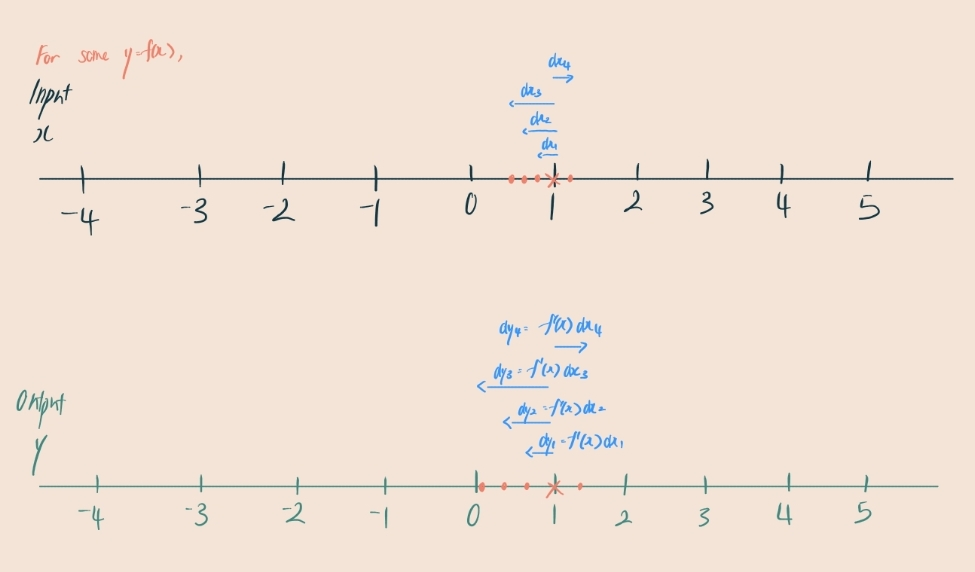
\includegraphics[width=0.8\textwidth, keepaspectratio]{Images/image2.jpg}
    \caption{\( f'(x) \) scales \( dx \) to produce \( dy \), with \( dx \) moving only left or right on the number line.}
    \label{fig:galaxy}
\end{figure}

For a fixed point $x$, we can interpret the differential form geometrically:

\begin{itemize}
    \item $f'(x)$ represents a constant real-valued scaling factor.
    \item $dx$ is a 1D vector with $x$ as the origin.
    \item $dy$ is the result of stretching or squeezing $dx$ by $f'(x)$, originating at $y$.
\end{itemize}

For real-valued functions, there are only two directions where $dx$ can be taken, either left or right along the real number line.


\subsection{Complex Differentials}

Like real-valued functions, the derivative of a complex function $f(z)=u+vi$, where $z$ represents a complex input in the form $x + yi$, is defined as the limit:

\begin{equation}
    f'(z) = \lim_{h \to 0} \frac{f(z+h) - f(z)}{h}
\end{equation}

Here, since $h$ is a complex number, this limit must exist no matter which direction $h$ approaches zero in the complex plane. Like the real case, when $h$ is very small (but not zero), this difference quotient approximates $f'(z)$. This approximation becomes more accurate as $h$ approaches zero, which allows us to think about tiny linear changes using differentials. For a complex function, we can write this in differential form:

\begin{equation}
    \frac{df}{dz} = f'(z) \implies df = f'(z)dz
\end{equation}

where $df$ represents a tiny change in $f$ along the complex plane, $dz$ represents a tiny change in $z$ along the complex plane, and $f'(z)$ represents the derivative at point $z$.

\begin{figure}[htp]
    \centering
    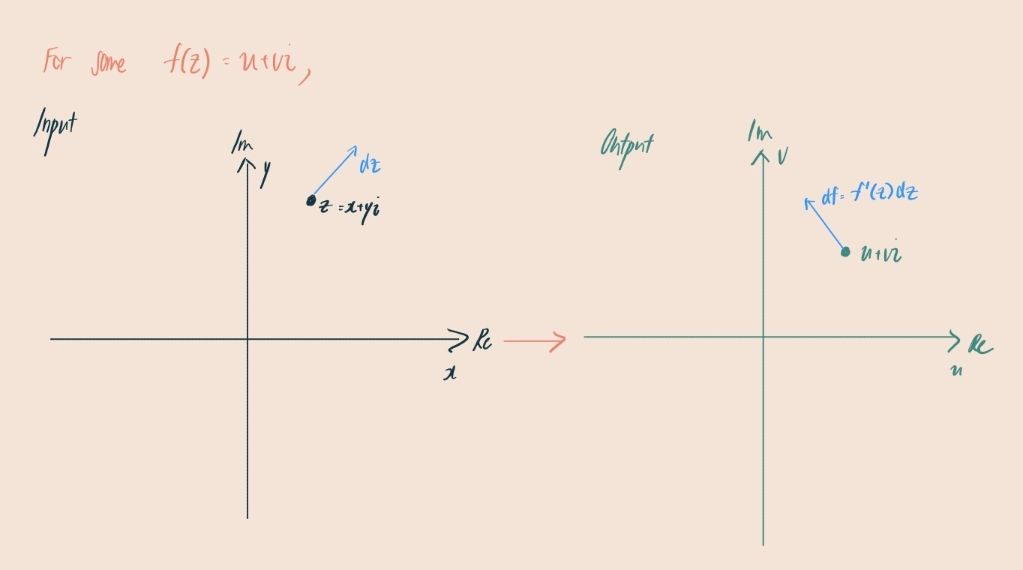
\includegraphics[width=0.8\textwidth, keepaspectratio]{Images/image3.jpg}
    \caption{\( f'(z) \) scales and rotates \( dz \) to produce \( df \) in the complex plane.}
    \label{fig:galaxy}
\end{figure}

For a fixed point $z = x+yi$, we can interpret the complex differential form similarly to the real case, with these key differences:

\begin{itemize}
    \item $f'(z)$ represents a constant complex-valued factor, $a+bi$. In polar form,  $re^{i\theta}$, $f'(z)$ combines both:
    \begin{itemize}
        \item a scaling factor, $r$ (the modulus)
        \item a rotation by angle $\theta$
    \end{itemize}
    \item In the complex plane:
    \begin{itemize}
        \item $dz$ is a 2D vector with $z$ as the origin.
        \item $df$ is a scaled and rotated 2D vector based on $f'(z)$, originating at $f$.
    \end{itemize}
\end{itemize}

\subsection{Holomorphicity}

\begin{figure}[H]
    \centering
    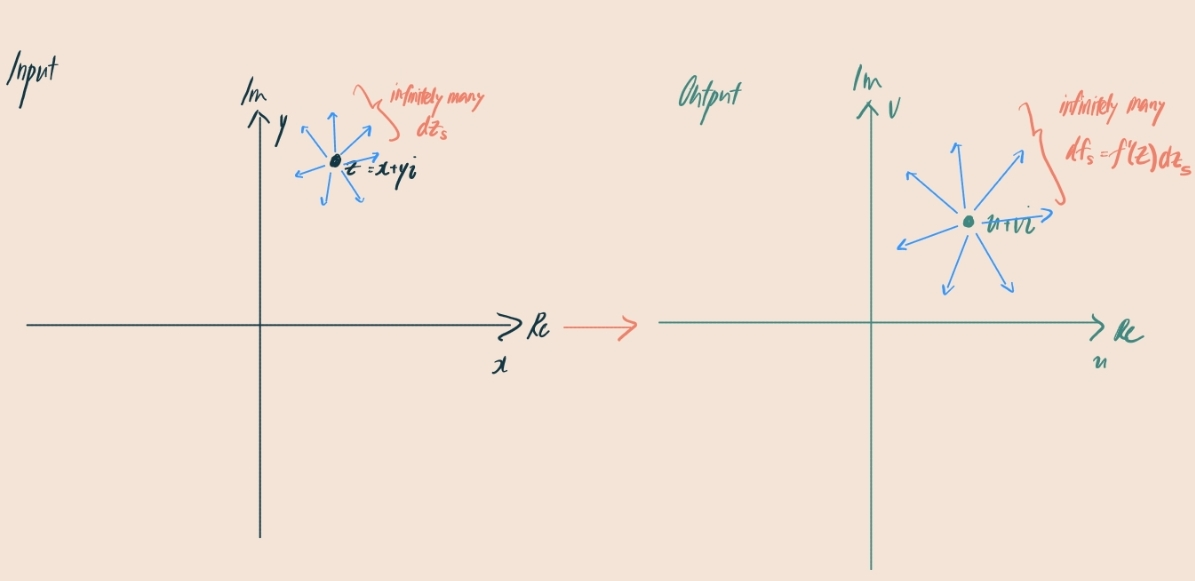
\includegraphics[width=0.8\textwidth, keepaspectratio]{Images/image4.jpg}
    \caption{\( dz \) can take infinitely many directions in the complex plane, forming a neighborhood around \( z \).}
    \label{fig:galaxy}
\end{figure}

In the complex case, unlike the real case where $dx$ can be taken in only two directions, there are infinitely many directions that $dz$ can take. The region these vectors collectively form is called the neighborhood of the specific point $z$. For a function to be complex differentiable, every image from $dz$ to $df$ in the neighborhood of $z$ must have the same scaling and rotating factor determined by $f'(z)$. Functions that are complex differentiable are called \textbf{holomorphic functions} (also known as \href{https://mathworld.wolfram.com/AnalyticFunction.html}{analytic functions}) at that point.

\begin{figure}[H]
    \centering
    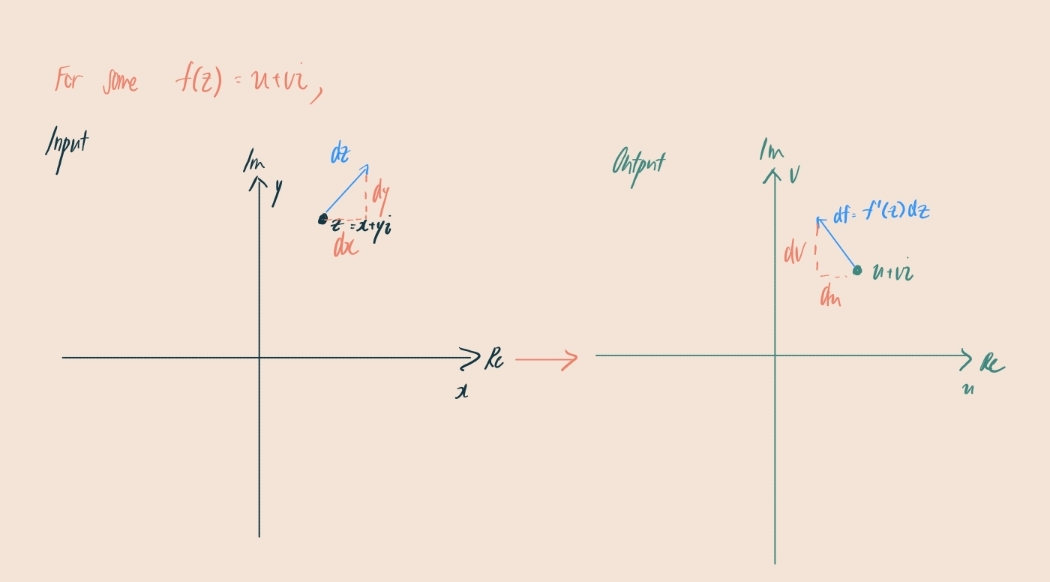
\includegraphics[width=0.8\textwidth, keepaspectratio]{Images/image7.jpg}
    \caption{\( f'(z) \) must apply the same scaling and rotation to all \( dz \) in the neighborhood of \( z \).}
    \label{fig:galaxy}
\end{figure}

If taking $dz$ in different directions requires different scaling and rotation transformations to get the corresponding $df$ vectors, then $f'(z)$ cannot exist at that point, and that function is not complex differentiable there.

\subsection{Conformality}

\begin{figure}[H]
    \centering
    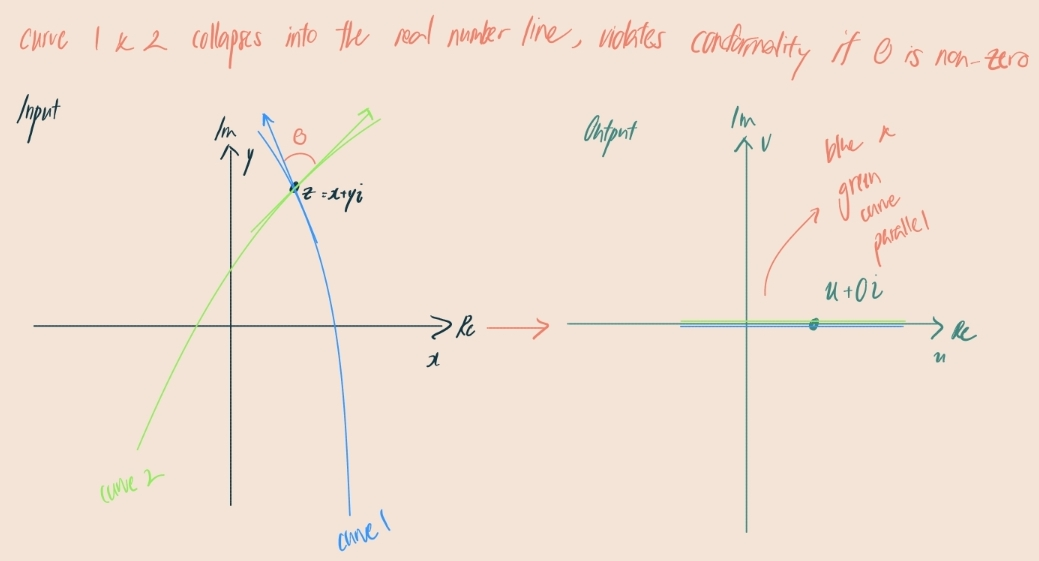
\includegraphics[width=0.8\textwidth, keepaspectratio]{Images/image8.jpg}
    \caption{A holomorphic function preserves the angle between intersecting curves when mapped from input to output space.}
    \label{fig:galaxy}
\end{figure}


For complex differentiability, the requirement that vectors must be rotated and scaled by the same amount leads to an important property called \href{https://mathworld.wolfram.com/ConformalMapping.html}{conformality}. At any point where a function is holomorphic, if two curves intersect, the angle between them is preserved when they are mapped by the complex function $f(z) = u+vi$ from the input space to the output space.

\section{How to Determine if a Complex Function is Complex Differentiable?}

We will now explore a systematic way to determine if complex functions are complex differentiable.

\subsection{Cauchy-Riemann Equations}

\subsubsection{Transformation from $dz$ to $df$}

\begin{figure}[htp]
    \centering
    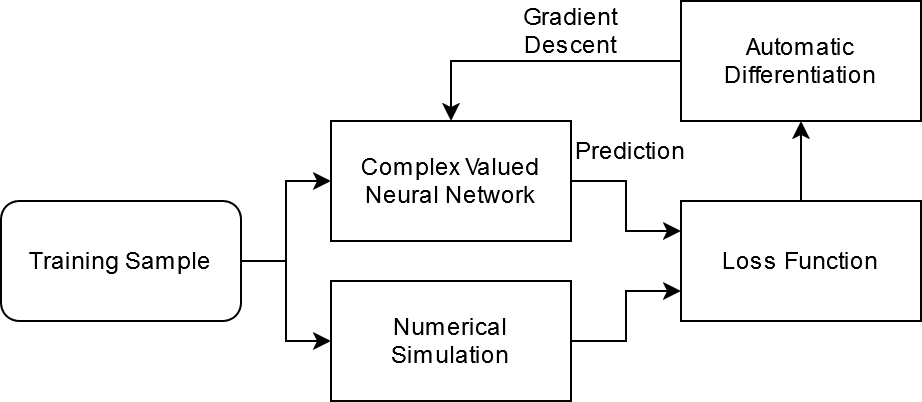
\includegraphics[width=0.8\textwidth, keepaspectratio]{Images/image9.jpg}
    \caption{\( dz \) decomposes into \( dx, dy \) in input space, while \( df \) decomposes into \( du, dv \) in output space.}
    \label{fig:galaxy}
\end{figure}

In the input space, an infinitesimal $dz$ can be decomposed into two linear components, $dx$ and $dy$. Similarly, in the output space, the corresponding image of $df$ can be decomposed into two linear components, $du$ and $dv$. Therefore, the transformation from $dz$ to $df$ can be written as:

\begin{equation}
\begin{bmatrix}
du \\
dv
\end{bmatrix} = J \cdot
\begin{bmatrix}
dx \\
dy
\end{bmatrix}
\end{equation}

where \(
\begin{bmatrix}
du \\
dv
\end{bmatrix}
\) represents the linear components that make up $df$, \(
\begin{bmatrix}
dx \\
dy
\end{bmatrix}
\) represents the linear components that make up $dz$, and $J$ represents a Jacobian matrix.

The components in the Jacobian matrix can be derived as follows:

\begin{itemize}
    \item For the $du$ component:
    \begin{equation}
        du = \Delta{u_{dx}}+\Delta{u_{dy}} \implies du = \frac{\partial{u}}{\partial{x}}dx+\frac{{\partial{u}}}{\partial{y}}dy
    \end{equation}
    since the change in $u$, $du$ comes from two parts, $dx$ and $dy$. Since $\Delta{u_{dx}}$ represents the change in $u$ when we vary $x$ while keeping $y$ fixed, and $\Delta{u_{dy}}$ represents the change in $u$ when we vary $y$ while keeping $x$ fixed, we can rewrite them using the partial derivatives $\frac{\partial u}{\partial x}$ and  $\frac{\partial u}{\partial y}$, respectively.
    
    \item Likewise, for the $dv$ component:
    \begin{equation}
        dv = \Delta{v_{dx}}+\Delta{v_{dy}} \implies dv = \frac{\partial{v}}{\partial{x}}dx+\frac{{\partial{v}}}{\partial{y}}dy
    \end{equation}
    since the change in $v$, $dv$ also comes from two parts, $dx$ and $dy$. We can rewrite $\Delta{v_{dx}}$ and $\Delta{v_{dy}}$ into partial derivatives for the same reason as $du$.
\end{itemize}

Thus, we can rewrite $J$, and the transformation from $dz$ to $df$ is:

\begin{equation}
\begin{bmatrix}
du \\
dv
\end{bmatrix} =
\begin{bmatrix}
\frac{\partial{u}}{\partial{x}} & \frac{\partial{u}}{\partial{y}} \\
\frac{\partial{v}}{\partial{x}} & \frac{\partial{v}}{\partial{y}}
\end{bmatrix}
\cdot
\begin{bmatrix}
dx \\
dy
\end{bmatrix}
\end{equation}

\subsection{Cartesian Form of the Complex Differential}

Using the complex differential $df = f'(z)dz$, and rewriting it in its Cartesian form:

\begin{equation}
du + dvi = (a+bi)(dx+dyi)
\end{equation}

The complex multiplication:$(a+bi)(dx+dyi) = (a \cdot dx - b \cdot dy) + (b \cdot dx + a \cdot dy)i$

can be represented as a $2 \times 2$ matrix with the first row corresponding to the real part and the second row corresponding to the imaginary part:

\begin{equation}
\begin{bmatrix}
a \cdot dx & -b \cdot dy \\
b \cdot dx & a \cdot dy
\end{bmatrix} =
\begin{bmatrix}
a & -b \\
b & a
\end{bmatrix}
\begin{bmatrix}
dx \\
dy
\end{bmatrix}
\end{equation}

Therefore, the \textbf{Cartesian form of the complex differential} can be expressed as:

\begin{equation}
\begin{bmatrix}
du \\
dv
\end{bmatrix} =
\begin{bmatrix}
a & -b \\
b & a
\end{bmatrix}
\cdot
\begin{bmatrix}
dx \\
dy
\end{bmatrix}
\end{equation}

\subsection{Equating the Transformation from $dz$ to $df$ and Cartesian Form of the Complex Differential}

Comparing both transformations:
\begin{equation}
\begin{bmatrix}
    a & -b \\
    b & a
\end{bmatrix} =
\begin{bmatrix}
    \frac{\partial{u}}{\partial{x}} & \frac{\partial{u}}{\partial{y}} \\
    \frac{\partial{v}}{\partial{x}} & \frac{\partial{v}}{\partial{y}}
\end{bmatrix}
\end{equation}

We obtain the \href{https://mathworld.wolfram.com/Cauchy-RiemannEquations.html}{Cauchy-Riemann equations}:
\begin{equation}
    \frac{\partial u}{\partial x} = \frac{\partial v}{\partial x}, \quad
    \frac{\partial u}{\partial y} = -\frac{\partial v}{\partial y}
\end{equation}

Using the Cauchy-Riemann equations is a systematic way to check whether a complex function is \textbf{complex differentiable}, but satisfying these equations alone is \textbf{not sufficient}. For a function to be differentiable at a point, the following three conditions must hold:

\begin{enumerate}
    \item The \textbf{partial derivatives} must exist in a \textbf{neighborhood} of the point.
    \item The \textbf{partial derivatives} must be \textbf{continuous} at the point.
    \item The \textbf{Cauchy-Riemann equations} must be satisfied at the point.
\end{enumerate}

See \href{https://complex-analysis.com/content/complex_differentiation.html}{this resource} for more details on sufficient conditions for differentiability.

\section{Complex to Real Functions, $C \rightarrow R$}

\subsection{Are $C \rightarrow R$ Functions Complex Differentiable?}

$C \rightarrow R$ functions map complex inputs to real outputs, with examples including $Re(z)$ and $Im(z)$. Geometrically, these functions collapse all complex inputs onto the real number line.

\begin{figure}[H]
    \centering
    \includegraphics[width=0.8\textwidth, keepaspectratio]{Images/image10.jpg}
    \caption{Mapping collapses complex inputs onto the real line, violating conformality.}
    \label{fig:galaxy}
\end{figure}

For a complex function to be holomorphic (complex differentiable), it must satisfy conformality - the preservation of angles between curves. However, when we consider two curves in the complex plane intersecting at a non-zero angle as illustrated above, their corresponding images must both lie on the real line. Consequently, the tangent vectors of these mapped curves must be parallel to the real axis, forcing the angle between them to be $0^\circ$. This clearly violates conformality, proving that such functions cannot be complex differentiable.

\subsection{Defining the Derivatives of $C \rightarrow R$ Functions}

We can alternatively write $C \rightarrow R$ functions as $f(x+yi)=u(x,y)$ where only the real value is retained for any given complex number input. While these functions cannot be complex differentiable (as they violate conformality), we can still analyze their rate of change by treating them as functions from $R^2 \rightarrow R$ using partial derivatives:

\begin{itemize}
    \item $\frac{\partial u}{\partial x}$ gives the rate of change in the $x$-direction.
    \item $\frac{\partial u}{\partial y}$ gives the rate of change in the $y$-direction.
\end{itemize}

This approach allows us to study how these functions change along specific directions, even though they fail to satisfy the stronger condition of complex differentiability which requires consistent behavior in all directions in the complex plane.

\vspace{0.5cm}

While complex differentiability imposes stronger conditions than real differentiability—requiring both \textbf{angle preservation} and \textbf{consistent behavior in all directions}—it also grants powerful properties. Complex differentiable functions, or \textbf{holomorphic functions}, are not only infinitely differentiable but also play a fundamental role in many mathematical and engineering applications.

\vspace{0.5cm}

One such application lies in \textbf{computational fluid dynamics (CFD)}, where complex differentiation helps model fluid behavior in aerodynamics. To understand the real-world impact of these mathematical concepts, we will explore their role in \textbf{aerospace engineering}, particularly in addressing turbulence.


\section{Mathematics of Rotor Turbulence}

Turbulence remains one of the most critical challenges in aerospace engineering, costing the airline industry up to \textbf{\$500 million annually} due to increased fuel consumption, aircraft wear, and maintenance costs. More importantly, turbulence contributes to \textbf{passenger injuries and structural stress}, demanding precise mathematical models to predict and mitigate its effects.

\begin{figure}[H]
    \centering
    \includegraphics[width=0.8\textwidth, keepaspectratio]{Images/video1.png}
    \caption{Modeling airflow over airfoils to analyze turbulence, lift, and aerodynamic efficiency.}
    \label{fig:galaxy}
\end{figure}

A major challenge in predicting and mitigating turbulence lies in its inherently chaotic nature, where small variations in airflow can escalate unpredictably.

Traditional CFD models struggle to accurately capture these rapid fluctuations, necessitating more advanced mathematical approaches to describe and differentiate turbulent flow patterns around aircraft rotors. Complex functions provide a powerful framework for modeling both the magnitude and directional changes of airflow, offering deeper insights into how turbulence forms and evolves.

\subsection{How is Rotor Flow Represented as Complex Functions}

In CFD for rotors, airflow around the blades is inherently \textbf{two-dimensional}, requiring both \textbf{magnitude and direction} to be tracked simultaneously. Instead of treating position and velocity as separate Cartesian coordinates, we represent them using \textbf{complex numbers}, a mathematical approach that provides a more natural and structured way to analyze flow behavior.

\subsubsection{Position:}

In 2D CFD modeling of a rotor, we define the position in the flow field as a complex number:

\begin{equation}
    z = x + iy
\end{equation}

where:

\begin{itemize}
    \item $x$ and $y$ are Cartesian coordinates in the plane of the rotor.
    \item $i$ represents the imaginary unit, which enables us to encode both spatial dimensions within a single mathematical object.
\end{itemize}

Using complex numbers for representing position is useful because it makes certain flow behaviors, like \textbf{rotation}, easier to describe mathematically. For example, when air rotates around the rotor, we can represent this motion simply by multiplying by a complex number $e^{i\theta}$ , which rotates the position by an angle $\theta$. In contrast, with Cartesian coordinates, we would have to use separate trigonometric equations for $x$ and $y$, making the math more complicated.

\vspace{0.2cm}

Similarly, differentiation and integration in the complex plane allow us to capture \textbf{both the rate of change and directionality} in a single operation, simplifying the analysis of how the rotor influences the surrounding airflow.

\subsubsection{Velocity:}

The velocity of airflow at any point is also inherently \textbf{two-dimensional}, consisting of both a speed and a direction:

\begin{equation}
    f(z) = u(x, y) + iv(x, y)
\end{equation}

where:

\begin{itemize}
    \item $u(x, y)$ = horizontal velocity component (e.g., forward/lateral airflow).
    \item $v(x, y)$ = vertical velocity component (e.g., rotational/induced flow).
\end{itemize}

This means that $f(z)$ tells us both the \textbf{speed and the direction} of the airflow at every point. The \textbf{magnitude} $|f(z)|$ of this function gives the actual speed of the airflow, while the \textbf{angle} $\arg(f(z))$ tells us which direction the air is moving.

\subsection{What Does Differentiating this Function Mean?}

To understand how airflow varies around a rotor, we take the derivative of $f(z)$, which provides:

\begin{itemize}
    \item \textbf{How fast the velocity changes} (i.e., acceleration effects).
    \item \textbf{How the flow direction evolves} around the rotor.
\end{itemize}

Differentiating a complex function means that we are capturing both \textbf{magnitude (speed) and directional changes} in the airflow in a single expression. This is essential in rotor design because it tells us how the air reacts to the movement of the blades.

\subsection{Challenges in Modeling Rotor Flow and Turbulence}

Turbulence is the chaotic and unpredictable behavior of fluid flow, where smooth motion suddenly breaks down into swirling vortices and eddies. Unlike laminar flow, where air moves in well-ordered layers, turbulence creates constantly changing velocity fields, making it difficult to model and predict. This instability is especially problematic in aerodynamics, where turbulent airflow over aircraft rotors is a major issue.

\begin{figure}[H]
    \centering
    \includegraphics[width=0.8\textwidth, keepaspectratio]{Images/collage.png}
    \caption{A. Laminar flow is smooth and orderly, while B. turbulence is chaotic and unpredictable}
    \label{fig:galaxy}
\end{figure}

\subsubsection{Why is Turbulence a Problem in CFD?}

\begin{itemize}
    \item \textbf{Unpredictable Flow Changes}: Small changes in rotor design can lead to large, nonlinear effects in airflow.
    \item \textbf{Breakdown of Differentiability}: In turbulent regions, the airflow does not behave smoothly—meaning direct differentiation of the velocity field can become meaningless.
    \item \textbf{Singularities and Discontinuities}: Flow separation (where air detaches from the blade) creates points where the function is not differentiable, leading to inaccurate results.
\end{itemize}

From a mathematical perspective, turbulence is difficult to handle because traditional differentiation relies on smooth, continuous changes in velocity. In an ideal, steady airflow, we can describe the velocity field using a complex function:$f(z) = u(x,y) + iv(x,y)$
where $u(x,y)$ represents the horizontal velocity component and $v(x,y)$ represents the vertical velocity component. This function is differentiable as long as it satisfies the Cauchy-Riemann equations:

\begin{equation}
    \frac{\partial u}{\partial x} = \frac{\partial v}{\partial y}, \quad \frac{\partial u}{\partial y} = -\frac{\partial v}{\partial x}
\end{equation}

These equations ensure that the function is \textbf{holomorphic}, meaning it behaves predictably and can be smoothly differentiated at every point in the flow field. In such cases, differentiation gives clear physical insights, such as the rate of change of velocity and the development of pressure fields.

\vspace{0.5cm}

However, turbulence breaks this structure. The presence of vortices, sudden shifts in velocity, and irregular motion cause the derivatives of $u(x,y)$ and $v(x,y)$ to become unstable. The Cauchy-Riemann equations fail because the partial derivatives no longer match as required. For example, if turbulence introduces random fluctuations modeled by an additional disturbance term $\epsilon(x,y)$, then the velocity field becomes:

\begin{equation}
    u(x,y)=-y+\epsilon(x,y), \quad v(x,y)=x+\epsilon(x,y)
\end{equation}

Differentiating these functions leads to inconsistent results:

\begin{equation}
    \frac{\partial u}{\partial x} - \frac{\partial v}{\partial y} \neq 0, \quad \frac{\partial u}{\partial y} + \frac{\partial v}{\partial x} \neq 0
\end{equation}

This violation of the Cauchy-Riemann equations means that the function is no longer differentiable in the traditional sense. At points where turbulence is extreme, differentiation gives erratic, non-physical values, making direct mathematical analysis impossible. The smooth, structured flow assumed in potential flow theory collapses, requiring alternative techniques such as numerical differentiation, finite difference methods, or complex-valued neural networks to approximate derivatives in these regions.

\subsection{Solutions for Modeling Turbulence in CFD - Complex Valued Neural Networks}

Research suggests that solving fluid dynamics numerically is \textbf{computationally expensive}. Replacing part of these simulations with neural networks can significantly reduce computational costs while maintaining accuracy.

\vspace{0.2cm}
One approach is to train a \textbf{neural network} to mimic the behavior of numerical simulations. This allows us to approximate fluid dynamics with \textbf{less computation} while preserving key characteristics of the simulation.
\vspace{0.2cm}

Since the system's state is described using \textbf{complex numbers}, it makes sense for our neural network to handle \textbf{complex-valued inputs, parameters, and outputs}. Such a model is called a \textbf{complex-valued neural network}. However, working with complex numbers introduces challenges in training the model.
\vspace{0.2cm}

To ensure the model replicates the numerical simulation accurately, we need a \textbf{loss function} that measures the difference between the model's output and the simulation results. In machine learning, the \textbf{loss function} is a \textbf{real-valued metric} that quantifies how far the model's output is from the expected value. The goal of training is to \textbf{minimize this loss}, improving the model's accuracy over time.

\begin{figure}[H]
    \centering
    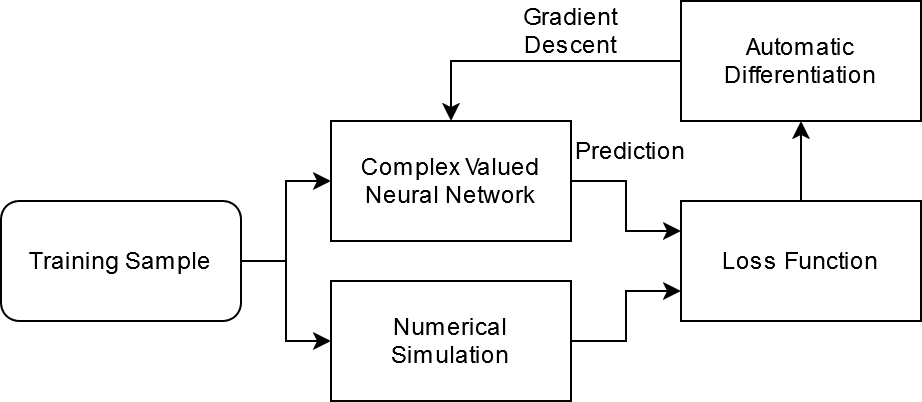
\includegraphics[width=0.8\textwidth, keepaspectratio]{Images/1image9.png}
    \caption{Workflow of loss function optimization: Measuring model accuracy and minimizing errors using gradient descent.}
    \label{fig:galaxy}
\end{figure}

The most common way to minimize loss is \textbf{gradient descent}. This method calculates the gradient of the loss function with respect to the model parameters. The gradient points in the direction where the loss increases the fastest. By adjusting the parameters in the opposite direction, we gradually reduce the loss. Repeating this process continuously improves the model.

\vspace{0.2cm}

However, since the \textbf{loss function is real-valued} while the \textbf{parameters are complex-valued}, standard differentiation does not apply. This is where the \textbf{Cauchy-Riemann equations} become relevant:

\begin{equation}
    \frac{\partial u}{\partial x} = \frac{\partial v}{\partial y}, \quad \frac{\partial u}{\partial y} = - \frac{\partial v}{\partial x}
\end{equation}

For a real-valued function with complex inputs, $v = 0$, so $\frac{\partial v}{\partial x} = \frac{\partial v}{\partial y}$. For the Cauchy-Riemann Equation to hold, $\frac{\partial u}{\partial x}$ and $\frac{\partial u}{\partial y}$ also need to be zero. This means that if this real-valued function is differentiable, it needs to be a constant. But obviously, the loss function cannot be a constant, so it is not differentiable, and we cannot take its gradient. Numeric differentiating methods will not work in this case either, since the value of numeric partial derivatives is likely to approach different values from different directions.

\vspace{0.5cm}

The simplest solution is to treat the \textbf{real and imaginary parts} of a complex parameter as separate real numbers. This allows us to compute their partial derivatives using standard real-valued algorithms. In this approach, a real-valued function with complex inputs is converted into a real-valued function with real inputs, making optimization possible with \textbf{real gradients} instead of complex ones.

\vspace{0.5cm}

Most auto-differentiation libraries, like \textbf{PyTorch} and \textbf{Zygote.jl}, use this method—and it works seamlessly.

\vspace{0.5cm}

To demonstrate this method, we crafted an example program that optimized the simplest model with complex-valued parameters. This program fits the Discrete Fourier Transformation of length 4, with randomly generated training samples and gradient descent. The Discrete Fourier Transformation is a complex-valued linear transformation that transforms a sequence of complex numbers into a new sequence of complex numbers of the same length. The program adjusts a matrix $A$ so that $A \vec{x}$ is the normalized Discrete Fourier Transform of $\vec{x}$.

\subsection{Implementation of Complex-Valued Neural Networks for Turbulence Modeling}

Below is a Julia implementation that optimizes a complex-valued neural network to fit the Discrete Fourier Transformation (DFT). This program trains a matrix $A$ such that $A \vec{x}$ approximates the normalized DFT of $\vec{x}$.

\begin{verbatim}
using Zygote
using DSP

# learning rate
const η = 1e-3
const n_samples = 10000

# update the parameters with gradient descent and return the loss
function gradient_descent!(loss_fn, input, output, params...)
    loss, grads = withgradient((x...)->loss_fn(input, output, x...), params...)
    for (param, grad) in zip(params, grads)
        param .-= η .* grad
    end
    loss
end

# generate a training sample and train the model with it
function train!(mat)
    n = size(mat, 1)
    # generate a training sample x
    x = randn(ComplexF64, n)
    # compute the normalized Discrete Fourier Transformation of x
    # as the expected output of the model
    y = DSP.fft(x) ./ (n^2)
    # define the function 
    loss_fn = (x, y, mat) -> sum(abs.(mat*x-y))
    # update the parameters
    gradient_descent!(loss_fn, x, y, mat)
end

# initialize a random matrix as the starting point
A = randn(ComplexF64, 4, 4)
# train the matrix to fit the fft
for _ in 1:n_samples
    train!(A)
end
display(A)
\end{verbatim}

Since the Discrete Fourier Transformation is a linear transformation on a sequence with finite length, it can be represented in a matrix form. The ideal matrix representing the normalized DFT is:

\begin{table}[h]
\centering
\renewcommand{\arraystretch}{1.2} % Adjust row spacing
\resizebox{\textwidth}{!}{ % Automatically scale table to fit width
\begin{tabular}{c c c c}
 0.0625+0.0im & 0.0625+0.0im & 0.0625+0.0im & 0.0625+0.0im \\
 0.0625+0.0im & 0.0-0.0625im & -0.0625+0.0im & 0.0+0.0625im \\
 0.0625+0.0im & -0.0625+0.0im & 0.0625+0.0im & -0.0625+0.0im \\
 0.0625+0.0im & 0.0+0.0625im & -0.0625+0.0im & 0.0-0.0625im \\
\end{tabular}
}
\caption{Ideal Matrix Representation}
\end{table}

After training with 10,000 samples, the value of $A$ is:

\begin{table}[h]
\centering
\renewcommand{\arraystretch}{1.2} % Adjust row spacing
\resizebox{\textwidth}{!}{ % Automatically scale table to fit width
\begin{tabular}{c c c c}
 0.062726-8.21333e-5im & 0.0628331+0.00041729im & 0.0625017+0.000997758im & 0.0628604-0.000887635im \\
 0.0624501-0.000367902im & 0.000354766-0.0623343im & -0.0611046+0.000437316im & -0.00102272+0.0629469im \\
 0.0629067+0.00056035im & -0.0635738-0.00040853im & 0.0618573+0.00185821im & -0.0626741+0.000263615im \\
 0.0616903-0.000789189im & -0.000445818+0.062586im & -0.0612135-0.000140184im & -0.000234437-0.0622612im \\
\end{tabular}
}
\caption{Trained Matrix Representation}
\end{table}

As seen from the output, the trained matrix $A$ closely approximates the ideal Discrete Fourier Transformation matrix, validating the effectiveness of using gradient descent for complex-valued optimization.

\section{Summary}

Through this blog post, we have:

\begin{itemize}  
    \item Developed a rigorous mathematical foundation for \textbf{complex differentiability}, emphasizing \textbf{geometric intuition} through \textbf{transformation properties} and \textbf{conformality constraints}.  
    \item Applied \textbf{complex differentiation} principles to \textbf{CFD}, particularly in analyzing \textbf{rotor turbulence}, a major challenge in aerospace engineering due to its \textbf{unpredictability} and computational complexity.  
    \item Investigated the role of \textbf{complex-valued neural networks (CVNNs)} in overcoming the limitations of traditional CFD methods, demonstrating their potential to enhance turbulence modeling and improve predictive accuracy.  
\end{itemize}

\section{Contributions}

This project was a collaborative effort, with each team member contributing expertise in different areas.

\begin{itemize}
    \item \textbf{Irwin} established the mathematical background for complex differentiability by focusing on geometric understanding.
    \item \textbf{Souvik} led the initial ideation of Computational Fluid Dynamics (CFD) applications, developed the CFD portion on position, velocity, and differentiation. He also developed Python code for generating graphs and sourced relevant video references to enhance visual explanations.
    \item \textbf{Meichi} played a key role in structuring the blog, ensuring logical flow, and contributed to the initial ideation of various potential applications of complex functions.
    \item \textbf{Zichen} led the complex-valued neural network (CVNN) section, exploring how CVNNs can address mathematical challenges in turbulence modeling.
\end{itemize}

Each contribution helped shape this blog on complex differentiation and its role in CFD.

\end{document}
